\documentclass[aspectratio=169,10pt]{beamer}
\usetheme{Madrid}
\usecolortheme{seahorse}
\usepackage{amsmath,amssymb,amsthm}
\usepackage{listings}
\usepackage{xcolor}
\usepackage{graphicx}

\graphicspath{{figures/}}

% Code formatting
\lstset{
  basicstyle=\ttfamily\scriptsize,
  commentstyle=\color{green!50!black}\itshape,
  keywordstyle=\color{blue}\bfseries,
  stringstyle=\color{red},
  numbers=left,
  numberstyle=\tiny,
  frame=single,
  breaklines=true,
  language=Python
}

% Theorem definitions
\theoremstyle{plain}
\newtheorem*{theorem*}{Theorem}
\newtheorem*{definition*}{Definition}
\newtheorem*{lemma*}{Lemma}
\newtheorem*{corollary*}{Corollary}

% Set footline
\setbeamertemplate{footline}[frame number]

\title{Chapter 5f: Approximation of General Mapping}
\subtitle{Fixed Point Theorems in Ordered Banach Spaces}
\author{Pathak - An Introduction to Nonlinear Analysis and Fixed Point Theory}
\date{2018}

\begin{document}

\begin{frame}
  \titlepage
\end{frame}

\begin{frame}{Table of Contents}
  \tableofcontents
\end{frame}

\section{5.7.1: Existence of a Characteristic Vector}

\begin{frame}{Definition 5.75-5.78: Fréchet Derivatives and Operators}
  \begin{definition*}[Fréchet Differentiability]
    A nonlinear operator $F : X \to X$ is Fréchet differentiable with respect to cone $K$ at $x_0$ if:
    $$F(x_0 + h) - F(x_0) = F'(x_0)h + w(x_0, h), \quad h \in K$$
    where $\lim_{h \in K, \|h\| \to 0} \frac{\|w(x_0, h)\|}{\|h\|} = 0$.
  \end{definition*}

  \vspace{1em}

  \begin{definition*}[Positive Operator]
    A linear operator $F : X \to X$ is:
    \begin{enumerate}
      \item \textbf{Positive} if $F(K) \subseteq K$
      \item \textbf{Strictly positive} if $F(\bar{K}) \subset K$ (interior)
      \item \textbf{Strongly positive} if $F(\bar{K}) \subseteq \text{int}(K)$
    \end{enumerate}
  \end{definition*}

  \vspace{0.5em}

  \textit{Characteristic vectors are eigenvectors of $F$ in cone $K$ with nonnegative eigenvalues.}
\end{frame}

\begin{frame}{Theorem 5.145: Krasnoselski's Characteristic Vector Theorem}
  \begin{theorem*}[Krasnoselski [345]]
    Let $T$ be a continuous linear positive operator mapping bounded subsets into compact sets.

    If $T^p u \geq \alpha u$ for some nonzero $u$ with $-u \notin K$, $u = v - w$ $(v,w \in K)$, and
    some $p \in \mathbb{N}$, then $T$ has at least one characteristic vector $x_0 \in K$ with:
    $$Tx_0 = \eta_0 x_0$$
    where $\eta_0 \geq p\sqrt{\alpha}$.
  \end{theorem*}

  \vspace{1em}

  \textbf{Key insight:} Characteristic vectors correspond to positive eigenvectors of the operator $T$.
\end{frame}

\begin{frame}[fragile]{Example 5.50: Multiple Fixed Points}
  \begin{example*}
    Consider $X = \mathbb{R}$ with $K = [0, \infty)$ and operator:
    $$Tx = x + \frac{\sin x}{2}, \quad x \geq 0$$

    This isotone operator has three fixed points:
    $$x \in \left\{0, \frac{\pi}{2}, \frac{3\pi}{2}\right\}$$
  \end{example*}

  \vspace{1em}

  \begin{center}
    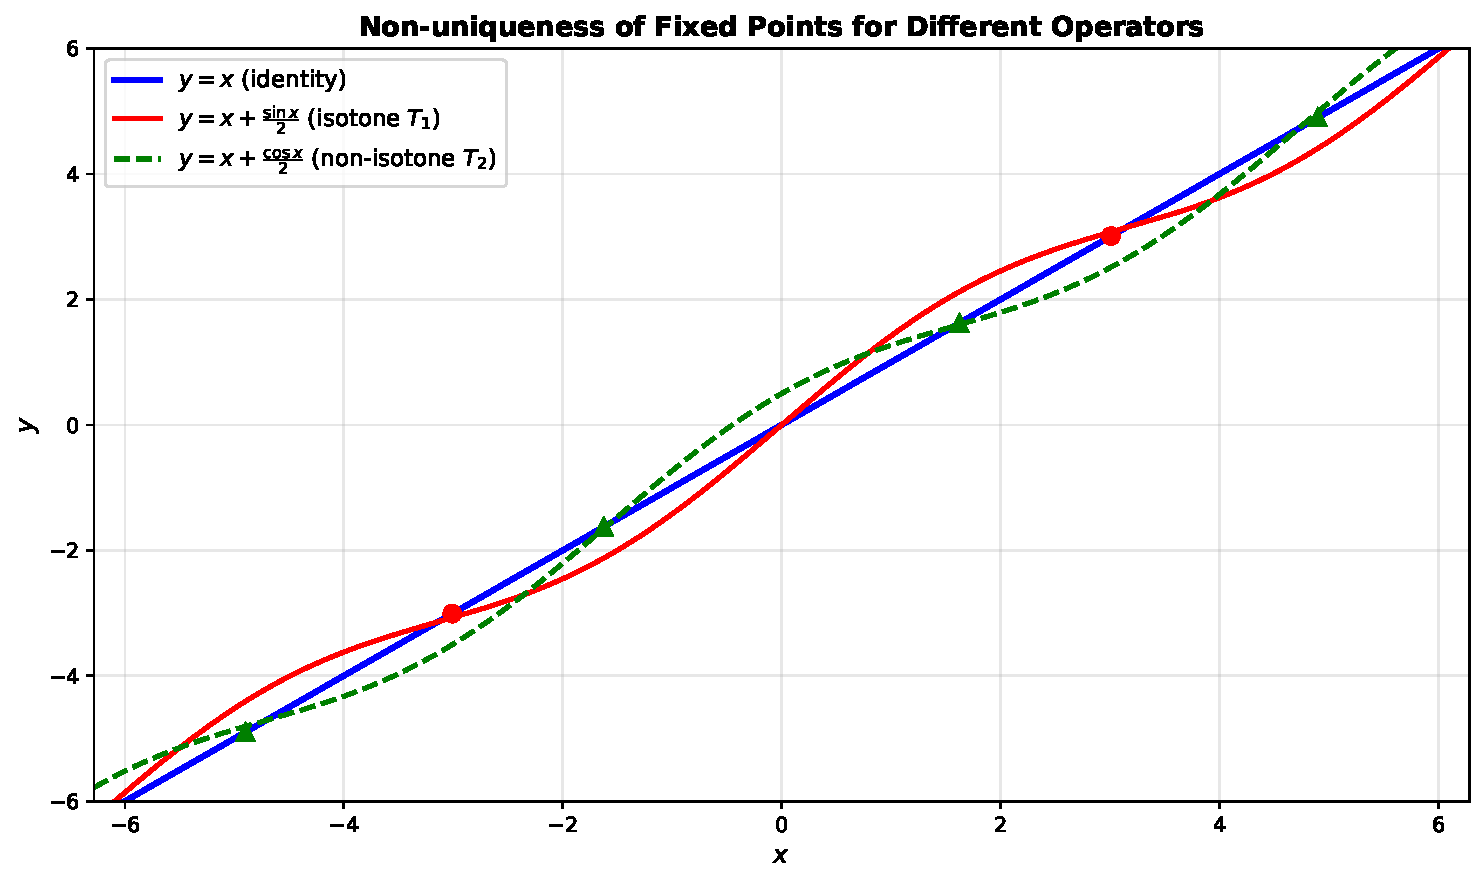
\includegraphics[width=0.7\textwidth]{nonunique_fixed_points.pdf}
  \end{center}
\end{frame}

\begin{frame}{Definition 5.80-5.81: Minimal/Maximal and Majorant}
  \begin{definition*}[Minimal/Maximal Fixed Points]
    A fixed point $x^*$ of $T: Y \to X$ is minimal if every fixed point $y$ satisfies $x^* \leq y$ $(x^* \geq y)$.
    There is at most one minimal (maximal) fixed point.
  \end{definition*}

  \vspace{1em}

  \begin{definition*}[Majorant/Minorant]
    A mapping $\bar{F}: Y \to X$ is a majorant of $F$ if $F(y) \leq \bar{F}(y)$ for all $y \in Y$.

    Minorants are defined by reversing the inequality.
  \end{definition*}

  \vspace{1em}

  \textbf{Spectral radius:} For linear operator $F: X \to X$,
  $$r(F) = \lim_{k \to \infty} \|F^k\|^{1/k}$$
\end{frame}

\section{5.7.1 (cont.): Multiple Fixed Point Theorems}

\begin{frame}{Theorem 5.150: Amann's Iterated Sequence}
  \begin{theorem*}[Amann [17]]
    Let $(X, K)$ be an ordered Banach space with $D$ order-convex. If
    $F: D \to X$ is increasing with $F(D)$ relatively compact, and
    there exist $\underline{y}, \bar{y} \in D$ with
    $\underline{y} \leq F(\underline{y})$ and $F(\bar{y}) \leq \bar{y}$,

    then $F$ has a minimal fixed point $\underline{x} \in (\underline{y}, \bar{y}) \cap D$ with:
    $$\underline{x} = \lim_{k \to \infty} F^k(\underline{y})$$
    The sequence $\{F^k(\underline{y})\}$ is increasing.
  \end{theorem*}

  \vspace{1em}

  \textbf{Proof idea:} Isotone property ensures monotone sequence convergence to fixed point.
\end{frame}

\begin{frame}{Corollary 5.32-5.33: Minimal and Maximal Fixed Points}
  \begin{corollary*}[Multiple Fixed Points]
    If hypotheses of Theorem 5.150 hold, then:
    \begin{itemize}
      \item $\underline{x} = \lim_{k \to \infty} F^k(\underline{y})$ (minimal fixed point)
      \item $\bar{x} = \lim_{k \to \infty} F^k(\bar{y})$ (maximal fixed point)
      \item Sequences $\{F^k(\underline{y})\}$ and $\{F^k(\bar{y})\}$ are monotone
    \end{itemize}
  \end{corollary*}

  \vspace{1em}

  \textbf{Key result:} Isotone mappings produce monotone iteration sequences.
\end{frame}

\begin{frame}{Theorems 5.151-5.153: Asymptotics and Nonisotone Operators}
  \begin{theorem*}[Spectral Radius Condition]
    If $F: K \to K$ is increasing, continuous, maps intervals to relatively compact sets,
    and has strongly positive Fréchet derivative $F'(0)$ with $r(F'(0)) > 1$,

    and continuous asymptotically linear majorant $\bar{F}$ with $r(F'(\infty)) < 1$,
    then $F$ has at least one fixed point in $\text{int}(K)$.
  \end{theorem*}

  \vspace{1em}

  \begin{theorem*}[Nonisotone Fixed Points]
    If $F$ has Fréchet and asymptotic derivatives with appropriate spectral radius bounds,
    then nonzero fixed points exist under continuity/compactness conditions.
  \end{theorem*}

  \vspace{0.5em}

  \textit{Generalizes fixed point theorems using asymptotic operator behavior.}
\end{frame}

\section{5.7.1 (cont.): Compression and Expansion}

\begin{frame}{Definition 5.82: Compression of a Cone}
  \begin{definition*}[Compression]
    A mapping $F: K \to K$ is a compression if $F(0) = 0$ and there exist $0 < r < R$ such that:
    \begin{enumerate}
      \item $Fx \not\preceq x$ for $x \in K$, $\|x\| \leq r$, $x \neq 0$ \quad (expansion near 0)
      \item $(1 + \varepsilon)x \not\preceq Fx$ for $x \in K$, $\|x\| \geq R$ \quad (compression near $\infty$)
    \end{enumerate}
  \end{definition*}

  \vspace{1em}

  \begin{center}
    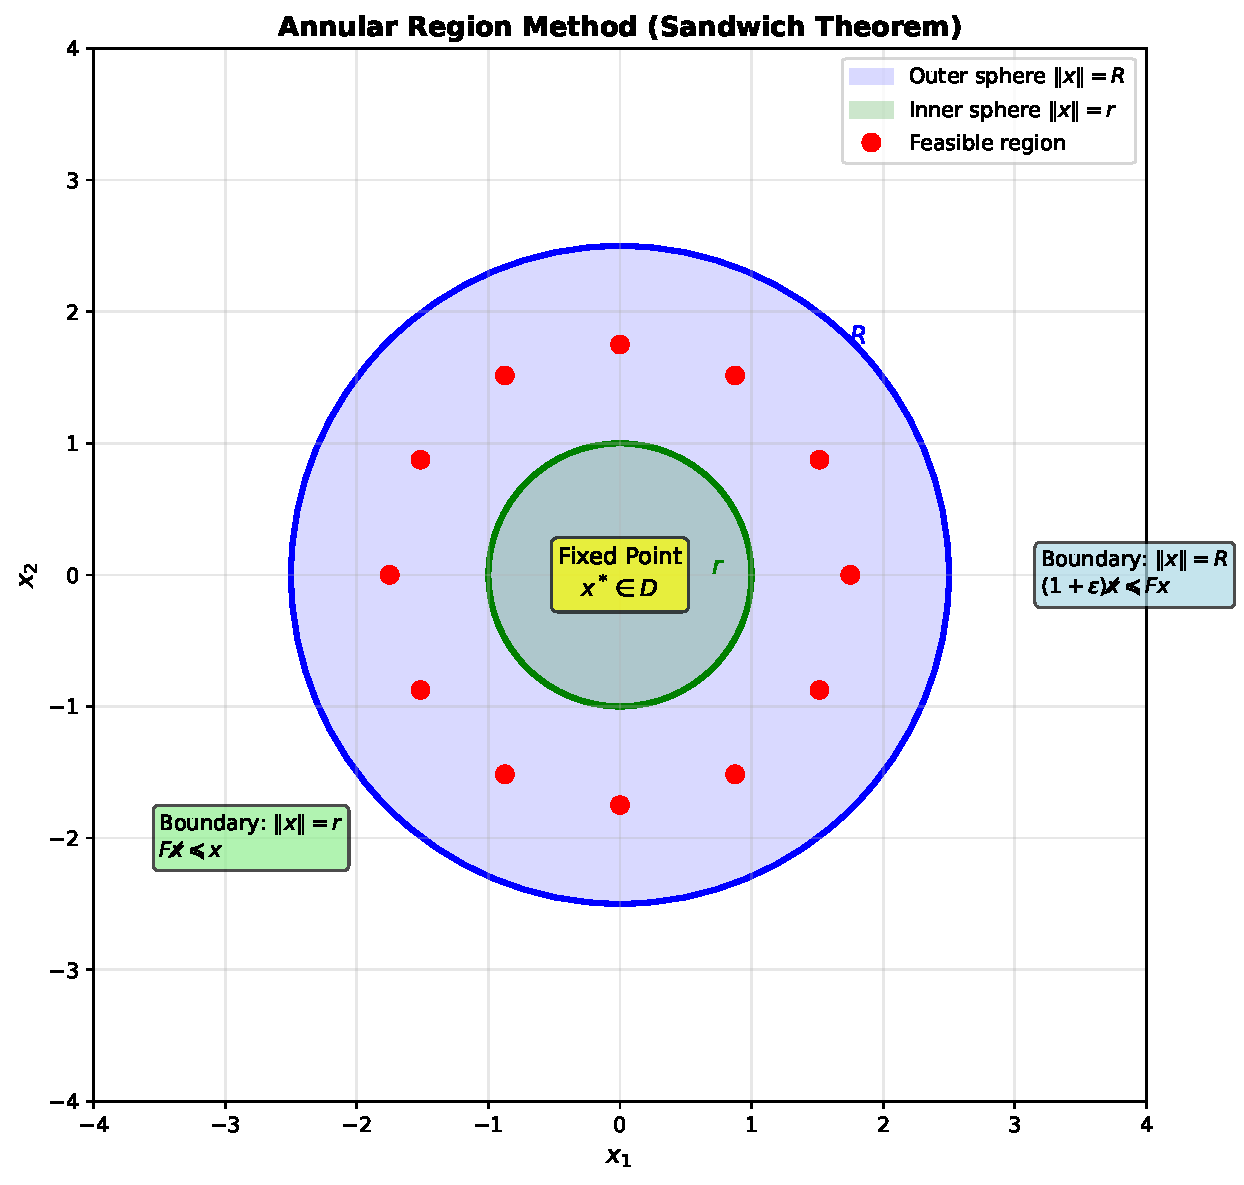
\includegraphics[width=0.6\textwidth]{annular_region.pdf}
  \end{center}

  \textbf{Krasnoselski [345]:} Compression operators have nonzero fixed points.
\end{frame}

\begin{frame}{Theorem 5.157-5.158: Leggett-Williams Fixed Points}
  \begin{theorem*}[Leggett-Williams [363]]
    Let $F: K_R \to K$ be continuous with $F(0) = 0$, mapping bounded sets
    into relatively compact sets. If:
    \begin{enumerate}
      \item For all $\varepsilon > 0$: $(1+\varepsilon)x \not\preceq Fx$ for $x \in K$, $\|x\| = R$
      \item There exists null sequence $\{u_n\}$ in $K_R$ such that if $x_n \to 0$ with
      $x_n \geq u_n$, there exists subsequence with $Fx_{n_k} \not\preceq x_{n_k}$
    \end{enumerate}

    then $F$ has a nonzero fixed point in $K_R$.
  \end{theorem*}

  \vspace{1em}

  \textbf{Extension:} Multiple fixed point theorems (Williams-Leggett [607]).
\end{frame}

\section{5.7.2: Partially Ordered Banach Spaces}

\begin{frame}{Definitions 5.83-5.89: Partially Ordered Space Operators}
  \begin{definition*}
    \begin{itemize}
      \item \textbf{Isotone:} $T(E) \to E$ preserves order: $x \preceq y \Rightarrow Tx \preceq Ty$
      \item \textbf{Compact:} $T(E)$ is relatively compact
      \item \textbf{Partially Continuous:} $||Tx - Ty|| < \varepsilon$ when $||x-y|| < \delta$ for comparable $x,y$
      \item \textbf{Partially Compact:} $T(C)$ relatively compact for all chains $C$
      \item \textbf{D-Lipschitzian:} $\|Tx - Ty\| \leq \varphi(\|x - y\|)$ for comparable elements
    \end{itemize}
  \end{definition*}

  \vspace{1em}

  \textbf{Compatibility condition:} Order relation $\preceq$ and metric $d$ compatible if
  nondecreasing sequences converging in metric imply pointwise convergence.
\end{frame}

\begin{frame}{Theorem 5.168: Dhage's Hybrid Fixed Point Theorem}
  \begin{theorem*}[Dhage [177]]
    Let $(E, \preceq, \|\cdot\|)$ be a regular partially ordered complete normed linear space.

    Let $\mathcal{P}, \mathcal{Q}: E \to E$ be nondecreasing operators where:
    \begin{enumerate}
      \item $\mathcal{P}$ is partially bounded and partially nonlinear $D$-contraction
      \item $\mathcal{Q}$ is partially continuous and partially compact
      \item There exists $x_0 \in E$ with $x_0 \preceq \mathcal{P}x_0 + \mathcal{Q}x_0$
    \end{enumerate}

    Then $\mathcal{P}x + \mathcal{Q}x = x$ has solution $x^* \in E$ with sequence
    $\{x_n\}_{n=0}^{\infty}$ (where $x_{n+1} = \mathcal{P}x_n + \mathcal{Q}x_n$)
    converging monotonically to $x^*$.
  \end{theorem*}
\end{frame}

\section{5.7.3: Weakly Contractive Mappings}

\begin{frame}{Weakly Contractive Mappings: Definition}
  \begin{definition*}[Weak Contraction]
    A self-map $T: X \to X$ is weakly contractive if for all $x, y \in X$:
    $$\|Tx - Ty\| \leq \|x - y\| - \psi(\|x - y\|)$$
    where $\psi: [0,\infty) \to [0,\infty)$ is continuous, nondecreasing with:
    \begin{itemize}
      \item $\psi(0) = 0$
      \item $\psi(t) > 0$ for all $t > 0$
      \item $\lim_{t \to \infty} \psi(t) = \infty$
    \end{itemize}
  \end{definition*}

  \vspace{1em}

  \textbf{Examples of} $\psi$: $\psi(t) = at$, $\psi(t) = \ln(1+t)$, $\psi(t) = \frac{t}{1+t}$.

  \vspace{0.5em}

  \textit{Generalizes Banach contraction: allows slower decay than linear.}
\end{frame}

\begin{frame}{Types of Weakly Contractive Mappings}
  \begin{definition*}[Weakly $(\varphi - \psi)$-Contractive]
    Type (I): For all $x,y \in X$,
    $$d(fx, fy) \leq \varphi(d(x,y)) - \psi(d(x,y))$$
    where $\varphi, \psi$ are continuous nondecreasing with:
    \begin{itemize}
      \item (C1) $\varphi(0) = \psi(0) = 0$
      \item (C2) $\varphi, \psi$ positive on $(0,\infty)$
      \item (C3) $\varphi(t) - \psi(t) < t$ for all $t > 0$
    \end{itemize}
  \end{definition*}

  \vspace{1em}

  \textbf{Type (II):} Same inequality with conditions (D1)-(D3) where $\psi$ is nonincreasing.

  \vspace{0.5em}

  \textit{Key advantage:} Existence without uniqueness assumption (some theorems).
\end{frame}

\begin{frame}{Theorem 5.169-5.171: Weakly Contractive Fixed Points}
  \begin{theorem*}[Harjani-Sadarangani [267]]
    If $(X, d)$ is complete metric space and $f: X \to X$ is continuous, nondecreasing with
    $$d(fx, fy) \leq d(x,y) - \psi(d(x,y)) \quad \text{for } x \geq y$$
    where $\psi$ satisfies (C1)-(C3), and exists $x_0 \in X$ with $x_0 \preceq f(x_0)$,
    then $f$ has a fixed point.
  \end{theorem*}

  \vspace{0.5em}

  \begin{theorem*}[Type (II) Version]
    Same conclusion holds for conditions (D1)-(D3) with $\psi$ nonincreasing.
  \end{theorem*}

  \vspace{1em}

  \textbf{Proof strategy:} Show $\{\rho_n\}$ sequence of distances is decreasing and converges to 0.
\end{frame}

\begin{frame}{Theorem 5.172-5.175: Uniqueness Conditions}
  \begin{theorem*}[Uniqueness in Ordered Sets]
    Under hypotheses of Theorem 5.171 with conditions:
    \begin{enumerate}
      \item (SC1) Every pair has lower or upper bound
      \item (SC2) Sequential comparability property
      \item (SC3) $f$ maps comparable elements to comparable elements
    \end{enumerate}

    Then fixed point is unique.
  \end{theorem*}

  \vspace{1em}

  \begin{example*}[Non-uniqueness]
    $X = \{(1,0), (0,1)\} \subset \mathbb{R}^2$ with $\varphi(t) = \frac{2}{3}t + \frac{1}{3}t^2$,
    $\psi(t) = \frac{2}{3}t$ satisfies weak contraction conditions with two fixed points in $X$.
  \end{example*}
\end{frame}

\begin{frame}{Example 5.51: Chain Analysis}
  \begin{example*}
    Let $X = \mathbb{R}$ with usual order and $\mathcal{C} = \{0\} \cup \{\pm 2^{-n} : n \in \mathbb{N}\}$.

    Define $f(x) = \frac{1}{2}x$ for all $x \in \mathcal{C}$.

    Then $\mathcal{C}$ is a chain in $X$ and $(X,d)$ complete metric space. The mapping $f$ is:
    \begin{itemize}
      \item Nondecreasing on comparable elements
      \item Weakly $(\varphi - \psi)$-contractive with $\varphi(t) = \frac{2}{3}t + \frac{1}{3}t^2$,
            $\psi(t) = \frac{1}{3}t$
      \item Unique fixed point at $0 \in \mathcal{C}$
    \end{itemize}
  \end{example*}
\end{frame}

\section{5.7.1: Advanced Results}

\begin{frame}{Theorem 5.155-5.156: Multiple Fixed Point Methods}
  \begin{theorem*}[Three Distinct Fixed Points]
    If there exist points $\underline{y}_1 < \underline{y}_2 < \bar{y}_1 < \bar{y}_2$ such that:
    \begin{itemize}
      \item $\underline{y}_1 \leq F(\underline{y}_1)$, $F(\underline{y}_2) \leq \underline{y}_2$
      \item $\bar{y}_1 \leq F(\bar{y}_1)$, $F(\bar{y}_2) \leq \bar{y}_2$
      \item $F$ continuous, strongly increasing with relatively compact range
    \end{itemize}

    then $F$ has at least three distinct fixed points $x, x_1, x_2$ with
    $\underline{y}_1 \leq x_1 \leq \underline{y}_2$, $\bar{y}_1 \leq x_2 \leq \bar{y}_2$.
  \end{theorem*}

  \vspace{1em}

  \textbf{Corollary 5.34:} Under same conditions, $x_1 \ll x_2 \ll x_3$ (three ordered fixed points).
\end{frame}

\begin{frame}{Theorem 5.159-5.161: Fixed Points in Function Spaces}
  \begin{theorem*}[Function Space Fixed Points]
    Let $F: (0,c)_\infty \to (0,c)$ be continuous with relatively compact range.
    If there exist $a, b, d$ with $0 < a < b \leq c$ and closed $\Omega_1 \subseteq \Omega$ such that:
    \begin{itemize}
      \item $|Fx(t) - Fx(s)| \leq b - a$ for $x \in (0,c)_\infty$ and $t,x \in \Omega_1$
      \item $Fx(t) > a$ and $F(x(t)) > a$ when $a \leq x(s) \leq b$ and $s \in \Omega_1$
    \end{itemize}

    then $Fx = x$ with $x(t) > a$ for each $t \in \Omega_1$ has a solution.
  \end{theorem*}

  \vspace{1em}

  \textbf{Application:} Boundary value problems and periodic solutions.
\end{frame}

\begin{frame}{Theorem 5.162-5.163: Annular Region Theorems}
  \begin{theorem*}[Sandwich Method - Gustafson-Schmitt [260]]
    Let $D = \{x \in K : r \leq \|x\| \leq R\}$ (annular region).

    If $F: D \to K$ is continuous mapping bounded sets to precompact sets with:
    \begin{enumerate}
      \item $\|x\| = R, Fx = \eta x \Rightarrow \eta \leq 1$
      \item $\|x\| = r, Fx = \eta x \Rightarrow \eta \geq 1$
      \item $\inf_{\|x\|=r} \|Fx\| > 0$
    \end{enumerate}

    then $F$ has fixed point in $D$.
  \end{theorem*}

  \vspace{0.8em}

  \begin{theorem*}[Reversed Boundaries]
    Same conclusion when (i) and (ii) inequalities reversed.
  \end{theorem*}
\end{frame}

\begin{frame}[fragile]{Numerical Example: Fixed Point Iteration}
  \begin{example*}
    Consider $Tx = \sin(x) + 0.3x$ on $[0, 2]$ with $K = [0, \infty)$.
  \end{example*}

  \begin{lstlisting}
# Fixed point iteration
import numpy as np
import matplotlib.pyplot as plt

def T(x):
    return np.sin(x) + 0.3 * x

# Iteration
x = np.array([0.5])
for i in range(20):
    x = np.append(x, T(x[-1]))

# Check convergence
print(f"Fixed point approximation: {x[-1]:.6f}")
print(f"Verification T(x*) ≈ x*: {T(x[-1]):.6f}")
print(f"Error: {abs(x[-1] - T(x[-1])):.2e}")

# Convergence rate
rates = np.abs(np.diff(x))
print(f"Convergence rate: {rates[-1]/rates[-2]:.4f}")
  \end{lstlisting}
\end{frame}

\begin{frame}{Theorem 5.164-5.166: Asymptotic Derivative Methods}
  \begin{theorem*}[Spectral Radius Bounds]
    If $F: K \to K$ maps bounded sets to precompact sets, satisfies:
    \begin{enumerate}
      \item $Fx = \eta x \Rightarrow \eta \leq 1$ for $\|x\| = R$
      \item $Fz = \eta Fz \Rightarrow \eta < \infty$ for some $z \in K, \|z\| = R$
      \item Continuous asymptotically linear majorant with spectral radius $< 1$
    \end{enumerate}

    then $F$ has fixed point $u \in K$ with $r \leq \|u\| \leq R$.
  \end{theorem*}

  \vspace{1em}

  \begin{theorem*}[Fréchet Derivative Condition]
    If $F'(0)$ has eigenvector $h \in K$ with $\eta_0 > 1$ and $F'(\infty)$ has spectral radius $< 1$,
    then nonzero fixed point exists.
  \end{theorem*}
\end{frame}

\section{5.7.2: Advanced Partially Ordered Results}

\begin{frame}{Theorem 5.167: Agarwal-Regan Multivalued Result}
  \begin{theorem*}[Agarwal-Regan [6]]
    Let $E$ be Banach space, $C \subseteq E$ cone with $\mathcal{K}(C)$ family of nonempty
    compact subsets of $C$.

    If $A: \Omega_r \cap C \to \mathcal{K}(C)$ is upper semicontinuous compact map with
    one of conditions:
    \begin{enumerate}
      \item (A) $\|y\| \leq \|x\|$ for all $y \in A(x)$ and $x \in \partial\Omega_R \cap C$,
              and $\|y\| > \|x\|$ for $x \in \partial\Omega_r \cap C$
      \item (B) Inequalities reversed
    \end{enumerate}

    then $A$ has fixed point in $C \cap (\bar{\Omega}_R \setminus \Omega_r)$.
  \end{theorem*}

  \vspace{0.5em}

  \textit{Extends to multivalued operators and set-valued mappings.}
\end{frame}

\section{5.8: Fixed Point Theorems in Banach Algebra}

\begin{frame}{Definition 5.92-5.93: Contractions in Banach Algebra}
  \begin{definition*}[Nonlinear Contraction]
    A mapping $T$ on Banach space $X$ is nonlinear contraction if:
    $$\|Tx - Ty\| \leq \varphi(\|x - y\|)$$
    where $\varphi: \mathbb{R}_+ \to \mathbb{R}_+$ continuous with $\varphi(r) < r$ for $r > 0$.
  \end{definition*}

  \vspace{1em}

  \begin{definition*}[D-Lipschitzian]
    A mapping $T$ is D-Lipschitzian if there exists continuous nondecreasing
    $\varphi: \mathbb{R}_+ \to \mathbb{R}_+$ with $\varphi(0) = 0$ such that:
    $$\|Tx - Ty\| \leq \varphi(\|x - y\|) \quad \text{for all } x,y \in X$$
  \end{definition*}

  \vspace{1em}

  \textit{Every Lipschitzian is D-Lipschitzian; converse may not hold.}
\end{frame}

\begin{frame}{Theorem 5.176-5.177: Krasnoselski in Banach Algebra}
  \begin{theorem*}[Krasnoselski [346] - Famous Result]
    Let $S$ be closed, convex, bounded subset of Banach algebra $X$.

    If $A, B: S \to X$ are operators with:
    \begin{enumerate}
      \item $A$ is contraction
      \item $B$ completely continuous
      \item $Ax + By \in S$ for all $x,y \in S$
    \end{enumerate}

    then $Ax + Bx = x$ has solution in $S$.
  \end{theorem*}

  \vspace{1em}

  \begin{theorem*}[Burton [126] - Modification]
    Condition (c) can be replaced by weaker condition:
    $A$ contraction and $B: S \to X$ completely continuous.
  \end{theorem*}

  \vspace{0.5em}

  \textbf{Application:} Nonlinear integral equations.
\end{frame}

\begin{frame}{Key Theorems Summary Table}
  \begin{center}
    \begin{tabular}{|l|c|c|c|}
      \hline
      \textbf{Theorem} & \textbf{Space Type} & \textbf{Operator Type} & \textbf{Result} \\
      \hline
      5.145 (Krasnoselski) & Ordered Banach & Positive Linear & Characteristic Vector \\
      \hline
      5.150 (Amann) & Ordered Banach & Isotone & Minimal Fixed Point \\
      \hline
      5.155 & Ordered Banach & Increasing & Three Fixed Points \\
      \hline
      5.162 & Cone in Banach & Continuous & Annular Region \\
      \hline
      5.168 (Dhage) & P. Ordered & Hybrid & Solution of $\mathcal{P}x + \mathcal{Q}x = x$ \\
      \hline
      5.171-5.175 & P. Ordered & Weakly $(\varphi-\psi)$ & Unique Fixed Point \\
      \hline
      5.176 (Krasnoselski) & Banach Algebra & $A$ contr., $B$ c.c. & Solution in $S$ \\
      \hline
    \end{tabular}
  \end{center}
\end{frame}

\section{Geometric and Analytical Perspectives}

\begin{frame}{Cone Properties and Fixed Point Existence}
  \begin{center}
    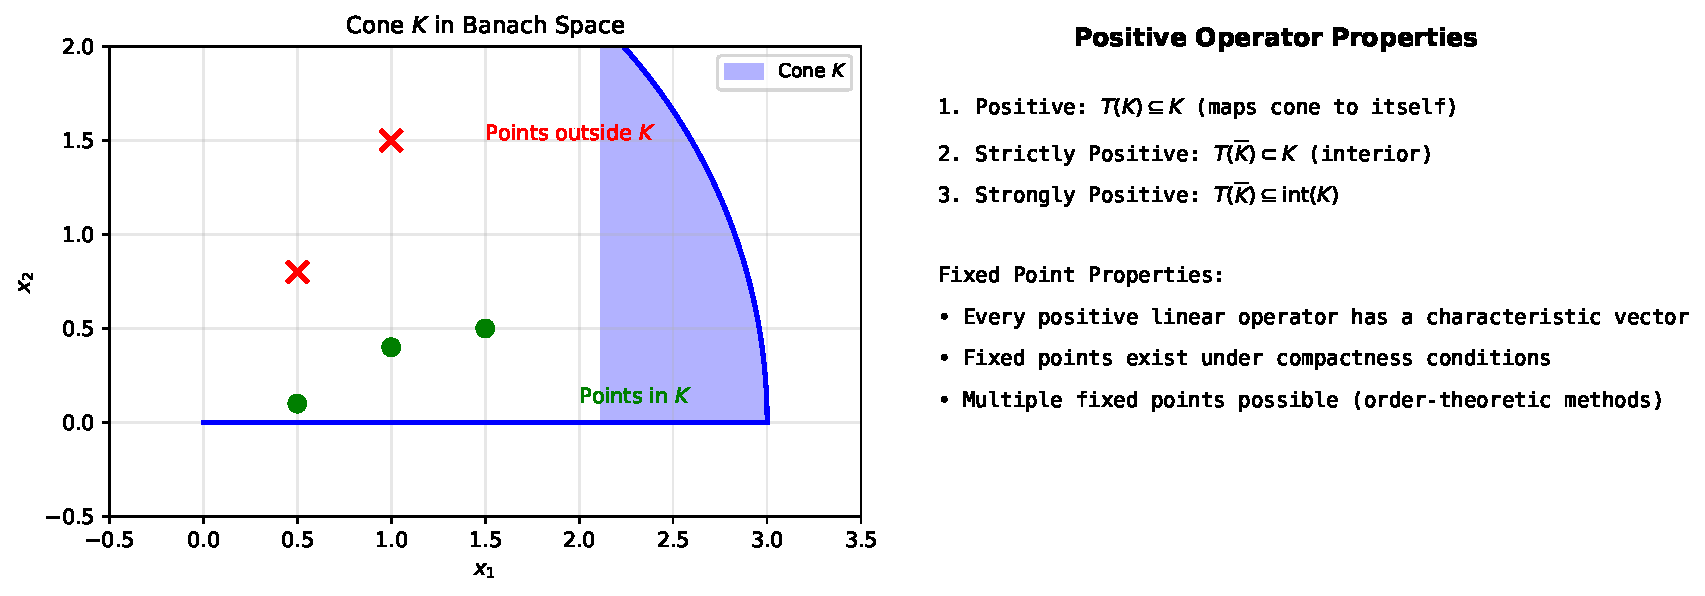
\includegraphics[width=0.8\textwidth]{cone_positive_operator.pdf}
  \end{center}

  \textbf{Geometric interpretation:}
  \begin{itemize}
    \item Positive operator maps cone into itself
    \item Fixed points lie in cone (order-theoretic nature)
    \item Compactness ensures convergent subsequences
  \end{itemize}
\end{frame}

\begin{frame}{Convergence Analysis}
  \begin{center}
    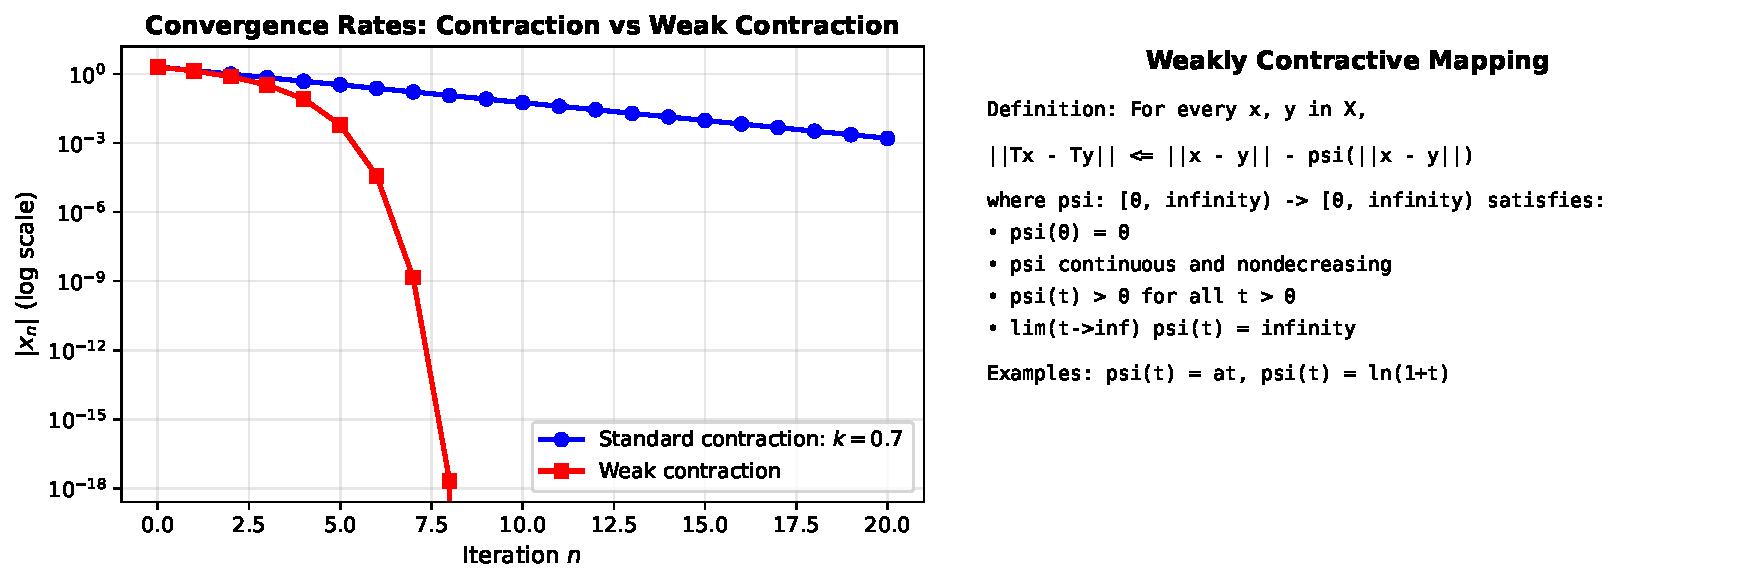
\includegraphics[width=0.9\textwidth]{weak_contractions.pdf}
  \end{center}

  \textbf{Weak vs. standard contractions:}
  \begin{itemize}
    \item Weak contraction: $\|Tx - Ty\| \leq \|x - y\| - \psi(\|x - y\|)$
    \item Allows slower convergence rates
    \item Useful for applications with nonlinear contractions
  \end{itemize}
\end{frame}

\begin{frame}{Spectral Radius and Stability}
  \begin{center}
    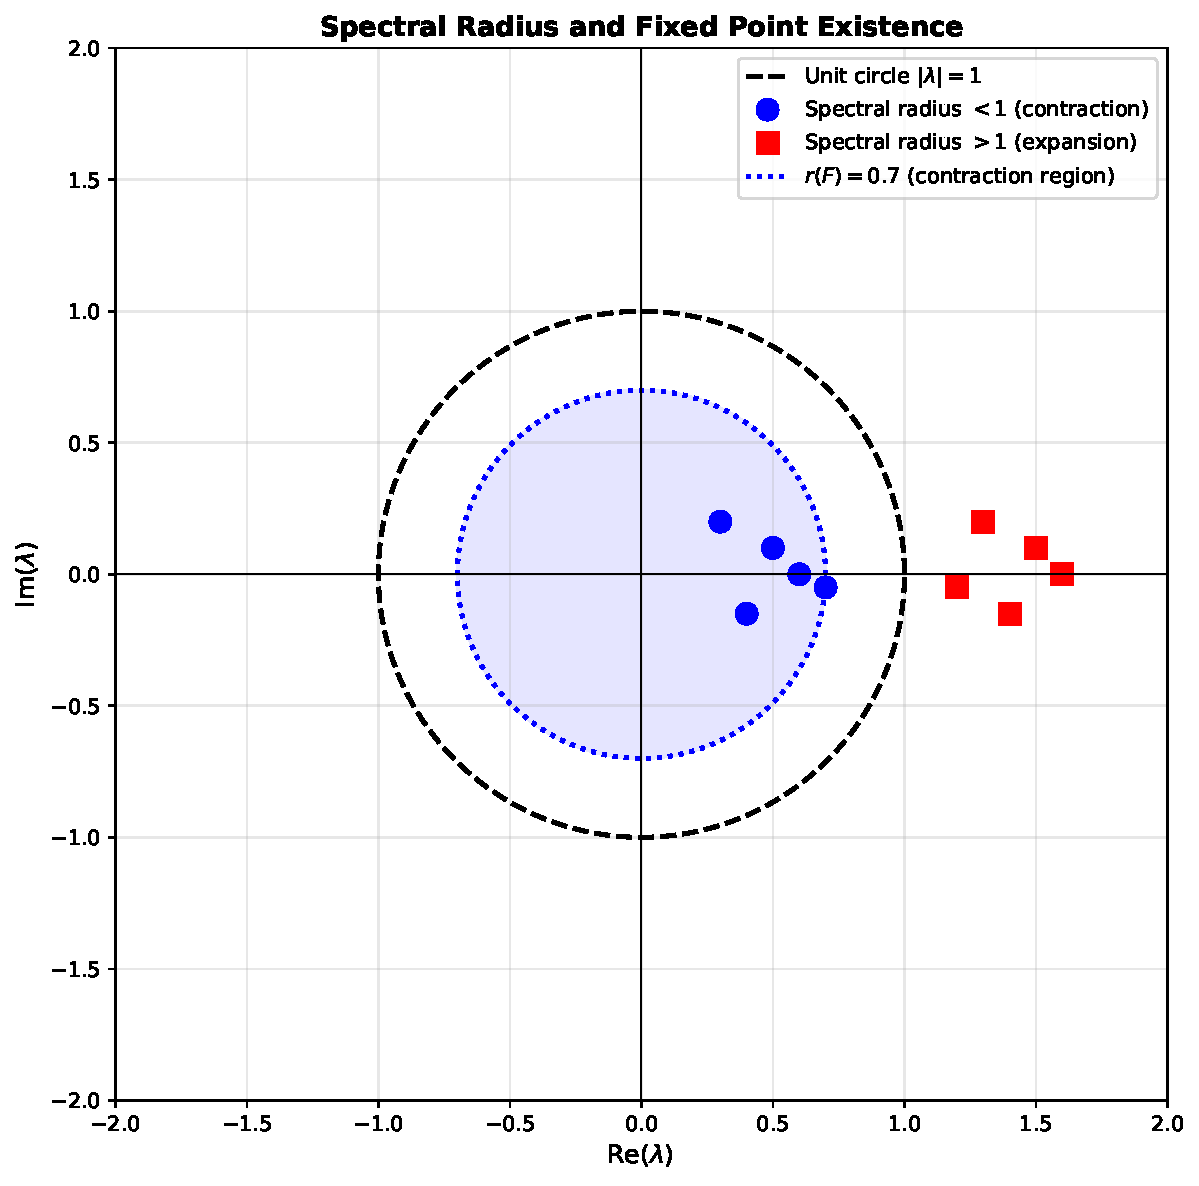
\includegraphics[width=0.8\textwidth]{spectral_radius.pdf}
  \end{center}

  \textbf{Key connections:}
  \begin{itemize}
    \item $r(F) < 1$: Contraction (exponential convergence)
    \item $r(F) = 1$: Critical case (slowest convergence)
    \item $r(F) > 1$: Expansion (no fixed points via contraction methods)
  \end{itemize}
\end{frame}

\begin{frame}{Partially Ordered Sets: Concepts and Structure}
  \begin{center}
    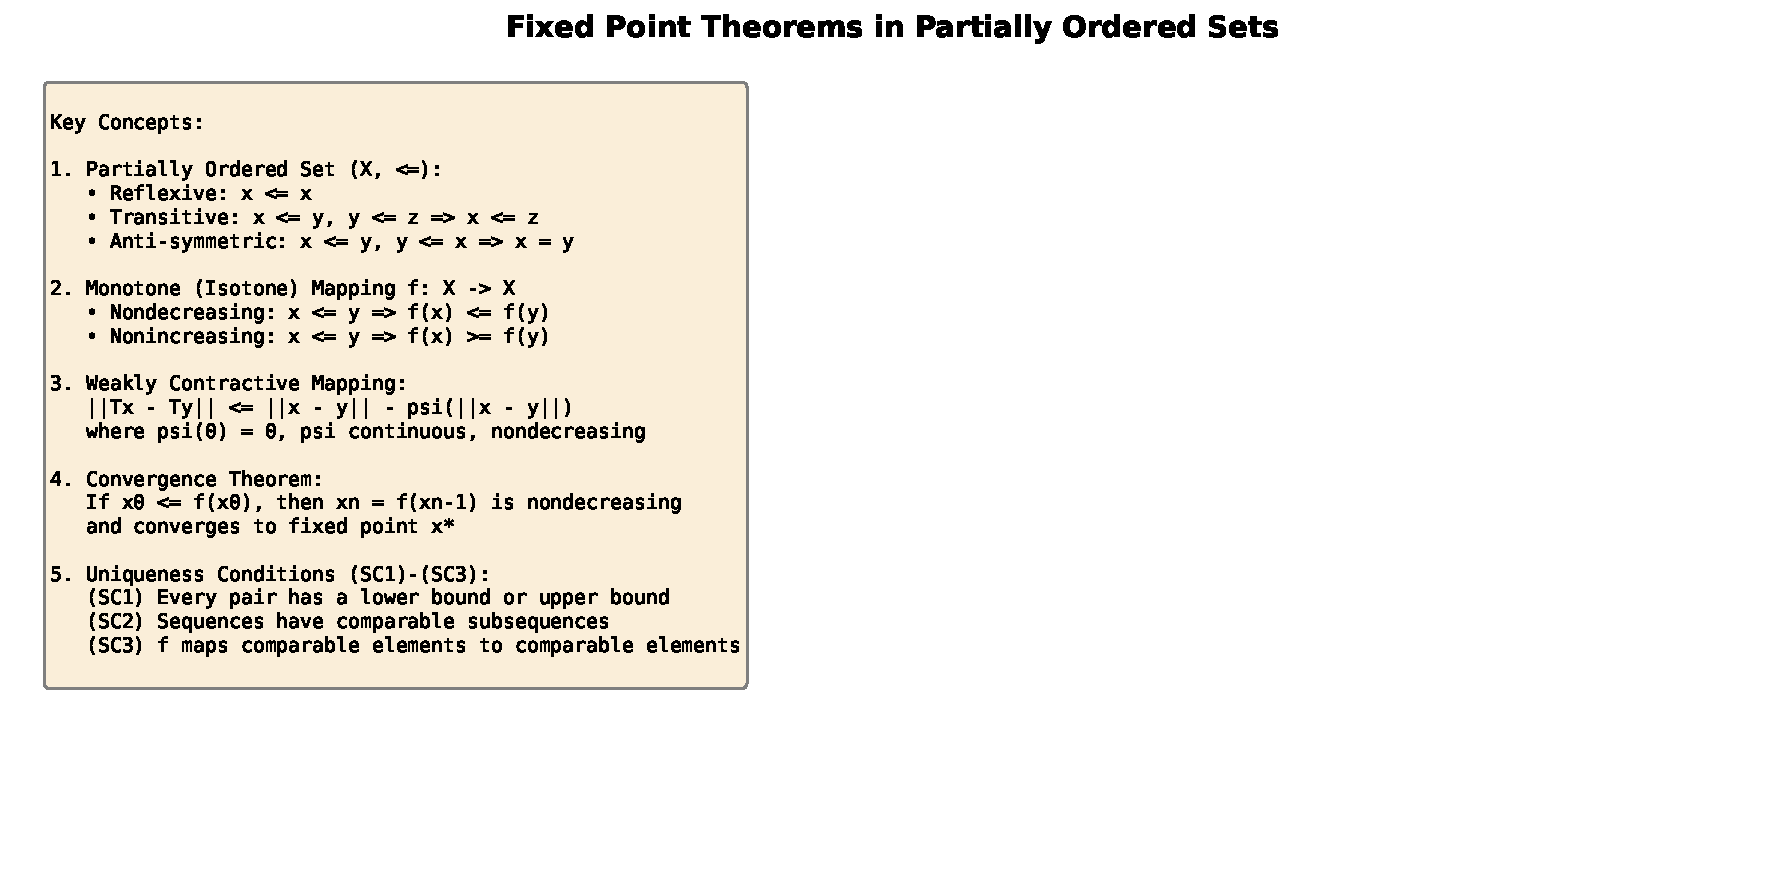
\includegraphics[width=0.95\textwidth]{partially_ordered_concepts.pdf}
  \end{center}
\end{frame}

\section{Applications and Extensions}

\begin{frame}{Applications to Boundary Value Problems}
  \textbf{Typical application:} Periodic boundary value problem
  \begin{align}
    x''(t) + f(t, x(t)) &= 0, \quad t \in [0, T] \\
    x(0) &= x(T), \quad x'(0) = x'(T)
  \end{align}

  \vspace{1em}

  \textbf{Fixed point formulation:}
  \begin{itemize}
    \item Green's function $G(t,s) \geq 0$ defines positive operator
    \item Integral operator: $Tx(t) = \int_0^T G(t,s) f(s, x(s)) ds$
    \item Theorems 5.150, 5.162, 5.168 guarantee solution existence
    \item Order-theoretic methods provide constructive iteration
  \end{itemize}

  \vspace{1em}

  \textbf{Advantage:} Weak differentiability assumptions; handles nonlinearities.
\end{frame}

\begin{frame}{Applications to Integral Equations}
  \textbf{Hammerstein integral equation:}
  $$x(t) = g(t) + \lambda \int_a^b K(t,s) f(s, x(s)) ds$$

  \vspace{1em}

  \textbf{Operator framework:}
  \begin{itemize}
    \item Write as $Fx = x$ with $Fx = Ax + Bx$
    \item $A$ contraction, $B$ compact in Krasnoselski method
    \item Application of Theorem 5.176
    \item For weakly contractive case: Theorems 5.171-5.175
  \end{itemize}

  \vspace{1em}

  \textbf{Key advantage:} Handles both singular and regular kernels via operator splitting.
\end{frame}

\begin{frame}{Convergence Theorems for Computation}
  \textbf{Iteration method:} $x_{n+1} = Tx_n$

  \vspace{1em}

  \textbf{Convergence guarantees:}
  \begin{enumerate}
    \item \textbf{Banach:} Linear convergence if $\|T'(x^*))\| < 1$
    \item \textbf{Monotone:} Guaranteed if $T$ isotone and $x_0 \leq Tx_0$
    \item \textbf{Weak contraction:} Guaranteed via distance decay $\rho_n \leq \varphi(\rho_{n-1}) - \psi(\rho_{n-1})$
    \item \textbf{Hybrid (Dhage):} Combination of linear and nonlinear components
  \end{enumerate}

  \vspace{1em}

  \textbf{Advantage of order-theoretic methods:}
  \begin{itemize}
    \item Provide bounds: $\underline{x} \leq x_n \leq x^* \leq \bar{x}_n$
    \item Guide computational algorithms
    \item Useful for error estimation
  \end{itemize}
\end{frame}

\section{Conclusion}

\begin{frame}{Chapter 5f: Main Takeaways}
  \textbf{Three main perspectives on fixed points:}

  \vspace{1em}

  \begin{enumerate}
    \item \textbf{Order-Theoretic:}
      \begin{itemize}
        \item Isotone/monotone operators
        \item Minimal/maximal fixed points
        \item Amann, Krasnoselski results
      \end{itemize}

    \item \textbf{Metric-Based:}
      \begin{itemize}
        \item Contraction principles
        \item Weakly contractive mappings
        \item Convergence rates
      \end{itemize}

    \item \textbf{Algebraic:}
      \begin{itemize}
        \item Banach algebra structure
        \item Krasnoselski hybrid method
        \item Operator splitting techniques
      \end{itemize}
  \end{enumerate}

  \vspace{1em}

  \textbf{Unified framework:} All methods apply to practical problems via appropriate operator construction.
\end{frame}

\begin{frame}[allowframebreaks]{References}
  \small

  \begin{thebibliography}{99}
    \bibitem{Pathak} Pathak, H.K. (2018). \emph{An Introduction to Nonlinear Analysis and Fixed Point Theory}. Springer.

    \bibitem{Amann} Amann, H. (1976). Fixed point equations and nonlinear eigenvalue problems. SIAM Review, 18(4).

    \bibitem{Krasnoselski} Krasnoselski, M.A. (1964). Positive solutions of operator equations. Groningen: Noordhoff.

    \bibitem{Dhage} Dhage, B.C. (2006). Hybrid fixed point theory in partially ordered normed linear spaces. J. Funct. Spaces Appl., 4(2).

    \bibitem{Dhage2} Dhage, B.C. (2009). Fixed point theorems in ordered Banach spaces and applications. Panamerican Math. J., 9(4).

    \bibitem{Harjani} Harjani, J., \& Sadarangani, K. (2009). Generalized contractions in partially ordered metric spaces. Fixed Point Theory Appl., 2009.

    \bibitem{Rhoades} Rhoades, B.E. (2001). Two fixed-point theorems for mappings satisfying a general contractive condition of integral type. Int. J. Math. Sci., 63.

    \bibitem{Burton} Burton, T.A. (1998). A fixed-point theorem of Krasnoselskii. Appl. Math. Lett., 11(1).

    \bibitem{Gustafson} Gustafson, G.B., \& Schmitt, K. (1983). Nonzero solutions of nonlinear systems of equations. J. Differential Equations, 52(2).

    \bibitem{LeggettWilliams} Leggett, R.W., \& Williams, L.R. (1979). Multiple positive fixed points of nonlinear operators on ordered Banach spaces. Indiana Univ. Math. J., 28(4).
  \end{thebibliography}
\end{frame}

\begin{frame}{End of Chapter 5f}
  \centering
  \Huge
  Fixed Point Theorems in Ordered Banach Spaces

  \vspace{2em}

  \Large
  Applications to approximation of general mappings

  \vspace{2em}

  \normalsize
  Complete theoretical framework for modern nonlinear analysis
\end{frame}

\end{document}
